\documentclass{beamer}
\beamertemplatenavigationsymbolsempty
\usepackage{amsmath, amssymb, hyperref, graphics, tikz}
%\usepackage{mathpazo, soul}



\newcommand{\C}{\mathbb{C}}
\newcommand{\Z}{\mathbb{Z}}
\newcommand{\R}{\mathbb{R}}
\newcommand{\N}{\mathbb{N}}
\DeclareMathOperator{\Real}{Re}
\DeclareMathOperator{\Imag}{Im}


\begin{document}

\begin{frame}{Seen on twitter -- ``Chaotic evil'' maths}
  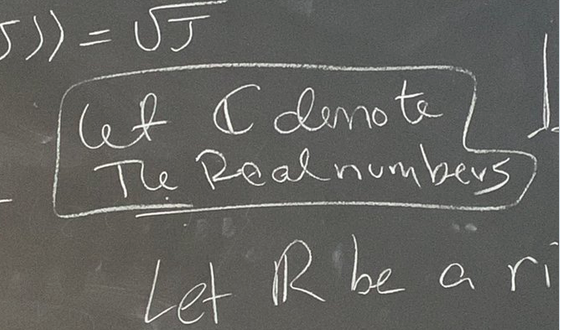
\includegraphics[width=\textwidth,height=0.8\textheight,keepaspectratio]{ChaoticEvil.png}
  
It's not "wrong", but it is painful. \\ Some definitions in the notes are similar...
\end{frame}


\begin{frame}{Types of Sets -- a topology taster}
The following Definition in the notes is NOT STANDARD USAGE.  
I won't use it.
    \begin{definition}[4.1 in notes]
    A \emph{neighbourhood} of $z_0\in\C$ is an open disc about $z_0$, i.e., it's of the form
    $$\{z\in\C : |z-z_0|<\delta\}$$
    for some $\delta>0$.
\end{definition}    
\begin{definition}[4.2 in notes. This definition is standard]
A set $D\subseteq \C$ is said to be \emph{open} if for each point $z_0\in D$ there's an open disc contained in $D$ and containing $z_0$.
\end{definition}
Easier to think in terms of pictures...
\end{frame}
\begin{frame}{``Can't be cut in two'' vs. ``Can get from place to place''}
Two possible intuitions behind being connected. 
\begin{definition}[Connected]
A subset $X\subseteq\C$ is \emph{connected} if we can't find two nonempty open sets $U,V\subset\C$ with $U\cap V=\emptyset$ and $X\subset U\cup V$.
\end{definition}
 Intuition: If $X\subset U\cap V$, then $X\cap U, X\cap V$ cuts $X$ into two pieces.
\begin{definition}[Path-connected]    
A subset $X\subseteq \C$ is called \emph{path-connected} if for any two points $x,y\in X$ we can find a path $\gamma\in X$ with initial point $x$ and final point $y$
\end{definition}
\begin{itemize}
    \item In general, path-connected $\implies$ connected, but not converse
\item If $X$ is open, $X$ is connected $\iff$ $X$ is path-connected.
\end{itemize}
\end{frame}

\begin{frame}{A little bit more}
Many of our Theorems are going to hold for nice open sets, so we develop shorthand for recording this.
\begin{definition}[4.4 in notes]
A non-empty, open, connected set is called a \emph{region}.
\end{definition}
\begin{definition}[4.5 in notes]
A region $D$ is said to be \emph{simply connected} if it has no `holes'; i.e., if every point in the interior of any simple contour in $D$ is contained in $D$.
\end{definition}
\begin{block}{Mathematical culture:}
We're implicitly using the Jordan Curve theorem -- that a simple curve closed in the plane has an inside and an outside.  
\end{block}
\begin{block}{Why is this hard?}
\end{block}
\end{frame}

\begin{frame}{Pick a point in the middle -- is it inside, or outside?}
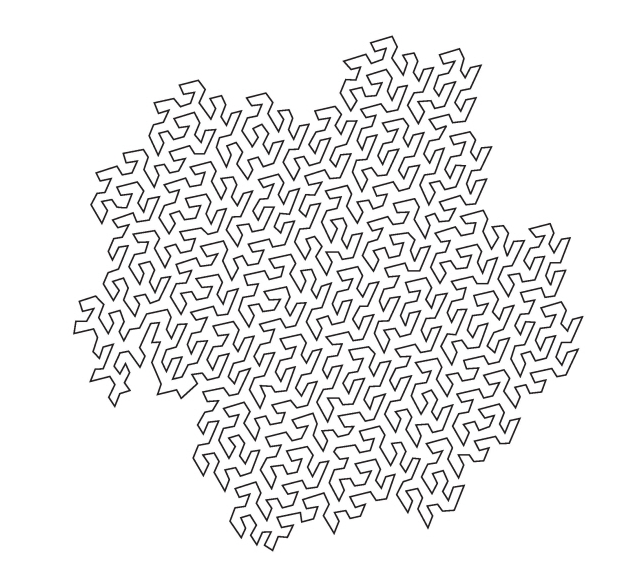
\includegraphics[width=\textwidth,height=0.8\textheight,keepaspectratio]{JordanCurveHard.png}

\end{frame}

\begin{frame}
  
\begin{center}

\Huge

\usebeamercolor[fg]{frametitle}
Clicker Session \\
Turning Point app or \\
ttpoll.eu 

\end{center}

\end{frame}


\begin{frame}{Actually computing line integrals}
$$\int_\gamma f(z)\text{d}z := \int_a^b f(z(t))z^\prime(t)\text{d}t$$
\begin{example}
Let $\gamma$ be the path that's a straight line from 0 to 1, and then a straight line from 1 to $2+i$.  Compute:
$$\int_\gamma \Real(z)\text{d}z$$
$$\int_\gamma \Imag(z)\text{d}z$$
$$\int_\gamma z\text{d}z$$
\end{example}
\end{frame}

\begin{frame}{The most important example}
Recall: $C_r(a)$ is the anti-clockwise circle of radius $r$ around $a$.  
\begin{block}{An mysterious computation:}
Let $n\in\Z$
$$\int_{C_r(a)}\frac{1}{(z-a)^n}\text{d}z=\begin{cases} 0 & n\neq 1 \\ 2\pi i & n=1\end{cases}$$
Independent of $a$ and $r$, works for $n$ negative, too!
\end{block}
\begin{block}{Coming attractions -- conceptual explanation!}
\begin{itemize}
    \item \emph{Antiderivatives} explain why the answer is zero unless $n=1$
    \item \emph{Cauchy's theorem} explains why it's independent of $r$
    \item \emph{Residue theorem} reduces \emph{any} integral to this computation!
\end{itemize}

\end{block}
\end{frame}


\end{document}

